\graphicspath{{figures/chapter2/}}
% Header
\renewcommand\evenpagerightmark{{\scshape\small Modeling metal organic frameworks}} 
\renewcommand\oddpageleftmark{{\scshape\small Chapter 2}}

%\renewcommand{\bibname}{References}

\hyphenation{}

\chapter[Modeling metal organic frameworks]%
{Modeling metal organic frameworks}
\label{ch2}

\begin{flushright}
\begin{quotation}
\textit{We are reaching the stage where the problems we must solve are going to become insoluble without computers. I do not fear computers. I fear the lack of them.} -- Isaac Asimov --
\end{quotation}
\end{flushright}
\npar
The understanding of catalytic processes in MOFs is a very challenging task. MOFs are materials of complex nature, and reactive processes in these materials are elusive and difficult to track on a purely experimental basis. Molecular simulations offer an alternative approach that starts from the construction of models that can explain, complement, and predict experiments. With growing computational power, computational models can aim at giving a more and more accurate description of materials at operating conditions, narrowing the gap between theory and experiment. Often, the structural properties and chemical transformations that take place on the active sites need to be investigated using a combination of multiple computational techniques, and the problems need to be tackled from different angles. 
In this chapter, an overview of the different computational methods that can be used to study reactive processes in MOFs will be given. 

\section{Framework topology}
A crucial decision when performing simulations lies in the choice of the model system, and what should be included in it. When choosing a model to represent the system under study, there is always a fine balance between accuracy and computational cost. 
On the one hand, it is crucial to use a computational model that captures all the relevant properties of the material and mimics the experimental structure as closely as possible. On the other, it is often convenient to approximate and neglect certain properties in favor of a larger scale description of the processes. The focus in this work are the active sites that can be used for catalysis, therefore an accurate electronic description of this region of the material is imperative. Nevertheless, the activity of these sites for chemical reactions can also be influenced by other factors, such as the pore size or functionalization. Therefore, to describe active sites in MOFs and other nanoporous materials, which can have rather large unit cells and non--periodic structural defects, the first question that needs to be asked is how to account for periodicity. Two conceptually different approaches can be used as shown below.

\subsection{Extended cluster model}
A very computationally efficient approach consists in neglecting periodicity and extracting a finite cluster of atoms from the periodic structure. This cluster model, displayed in Fig. \ref{fig:cluster-periodic}, contains the active sites and their surroundings but consists in a limited number of atoms, allowing to substantially decrease the computational cost. 
This allows both a more accurate treatment of the electronic structure, and a screening of different possible geometrical configurations of adsorbates, which is useful in the search for transition states (TS). Moreover, very efficient TS searching algorithms have been developed for such systems in Gaussian, the most widely used code for cluster calculations.
When extracting a cluster, particular attention has to be drawn to the termination of bonds and the charge compensation, that have to be done in the most realistic way. The rest of the crystal structure does not surround the external cluster atoms. Some of these atoms need to be fixed in order to mimic the periodic environment and prevent nonphysical deformations that would affect an estimation of the entropy \cite{DeWispelaere2018}.

\begin{figure}[!htbp]
	\centering
 	\includegraphics[width=1.0\textwidth]{cluster-periodic}
	\caption{Left: extended cluster model cut from the periodic structure of UiO--66. The cluster contains the active site, the brick and the linkers in the closest proximity to the active site. Right: representation of the unit cells containing the defect. In blue, the conventional 4--brick unit cell, in orange, the 2--brick unit cell used for the calculations. The two different bricks are highlighted in orange. The 10--fold coordinated brick has two terephthalate linkers missing.}
	\label{fig:cluster-periodic}
\end{figure}
\npar
Cluster calculations are an excellent way to benchmark and perform a first qualitative screening of reactions and possible configurations and have been for long the standard computational tool when studying reaction in nanoporous materials. However, they are not adequate to correctly describe complex reactive processes, where confinement effect of the pores and structural rearrangements can play an important role. The role of solvent in the pores can also be crucial for the outcome of a reaction and cannot be explicitly studied by cluster models. Periodic calculations resolve this shortcoming, and as computational power grows, the heterogeneous catalysis community is shifting towards these more expensive, however more accurate models. 

\subsection{Periodic model}
Periodic models, that fully take into account the periodicity of the crystal, enable to describe the whole topology of the framework. These calculations make use of periodic boundary conditions (PBC), which allow to simulate bulk phases with a limited number of atoms. In this model, the unit cell is replicated infinite times in each direction. When one atom disappears from one side of the unit cell it will reappear on the opposite side and each atom interacts with its neighbors in the same unit cell but also in the adjacent ones. Spurious interactions between the atoms can be avoided by applying a \textit{minimum image convention}, for which each atom interacts with its nearest neighbor or periodic image. In the case of long range interactions, such as the electrostatic ones, other techniques need to be used, such as Ewald summation \cite{Ewald1921}, where the potential is divided into a short range contribution, calculated in real space, and a long range contribution, calculated in reciprocal space using a Fourier transform. 
\npar
In the case of UiO--66, the conventional unit cell\cite{cavka2008new} contains 4 zirconium bricks (Fig. \ref{fig:periodic}, blue). In the calculations of this thesis, BDC linkers have been removed from the unit cell to introduce defects which are active sites in catalysis. Different amounts of missing linkers with different topologies have been considered \ref{fig:periodic}. An interesting topology is the one denoted as type 6 in the work of Rogge et al.\cite{rogge2017metal} that is characterized by a channel which offers good perspectives for the diffusion of guest molecules. This unit cell (displayed in blue in Fig. \ref{fig:periodic}) can be reduced by symmetry to a 2--brick unit cell (in orange, Figure \ref{fig:cluster-periodic}) which offers the best compromise between accuracy and computational cost. This reduced unit cell is used in most of the calculations performed in this thesis. In \textbf{PAPER I} we show that for catalytic purposes, the free energy differences calculated for the same chemical processes on the two unit cells is negligible, therefore the 2--brick unit cell represents a good model system. When modeling disorder, however, periodicity decreases and bigger unit cells have to be taken into account. For this reason, in \textbf{PAPER IV}, we studied defective 4--bricks unit cell with missing linkers ranging from zero to three. 

\begin{figure}[!htbp]
	\centering
 	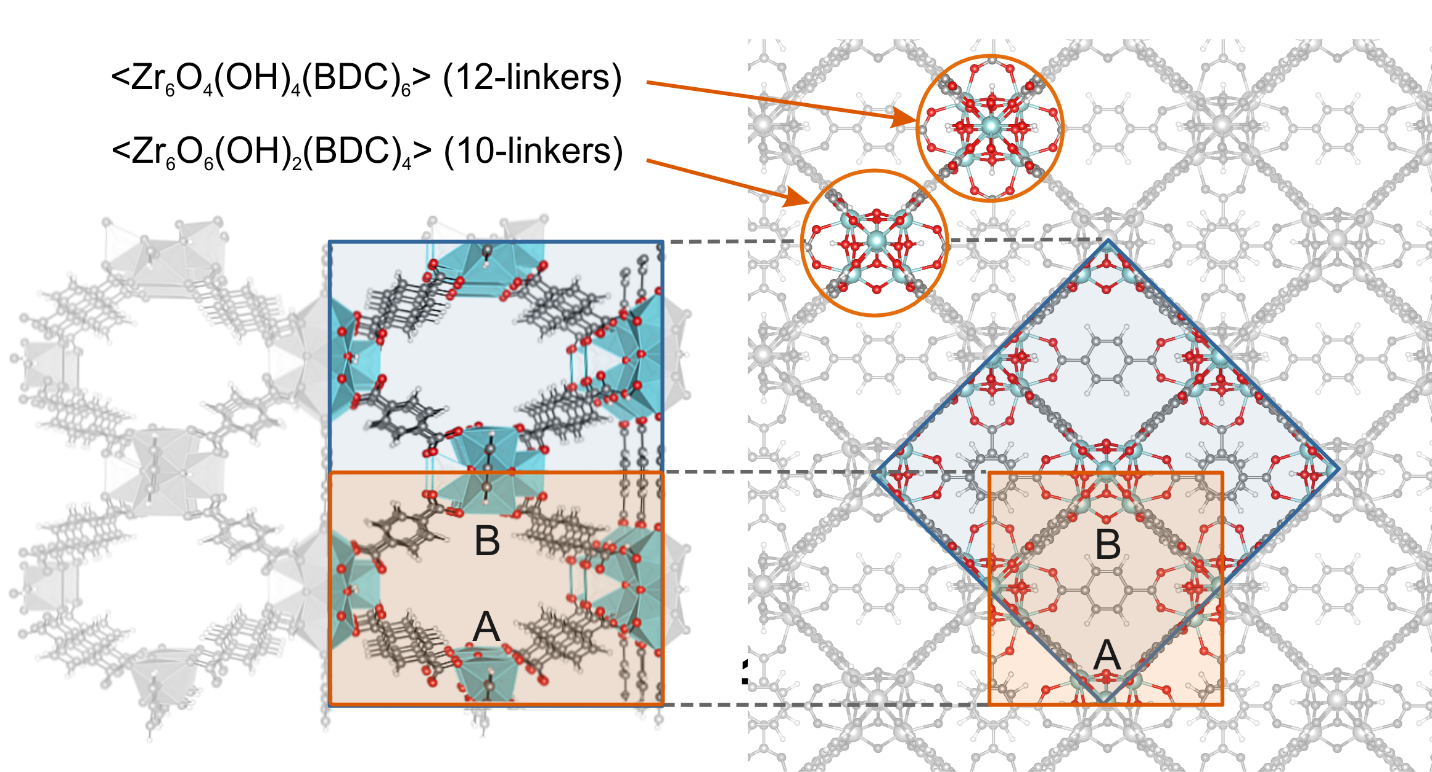
\includegraphics[width=1.0\textwidth]{periodic}
	\caption{Representation of the different ways to remove up to three linkers from a 4--brick UiO-66 unit cell}
	\label{fig:periodic}
\end{figure}

\section{Theoretical methods}
\subsection{Electronic energy methods}
A basic quantity to study any chemical or physical transformation is the potential energy surface (PES), which is a function of the coordinates of all the atoms of the system. The PES is always the reference quantity in our simulations and every atomic configuration can be represented as a point in this hypersurface, with a given value of potential energy (Figure \ref{fig:BO-approx}).
\npar
Ideally, by calculating the value of the PES for each atomic configuration we can obtain all information on the system and on the transformations that can occur. However, the complexity of this surface escalates quickly with the number of atoms, and the sampling of its relevant regions represents the main challenge of molecular simulations. The information gained by exploring the PES is tightly connected to the experimental observables. Statistical physics acts like a bridge between the microscopic insight that is gained through molecular simulations and the macroscopic properties which are measured experimentally. In principle, all macroscopic properties of a system can be derived from its wavefunction. To calculate it, the stationary Schr\"{o}dinger equation is solved: 
\[
\hat{H}\left\vert\psi\right\rangle = E\left\vert\psi\right\rangle
\]

where $\psi$ is the wavefunction, $\hat{H}$ is the Hamiltonian of the system, and $E$ is the total energy. The resolution of this equation is at the heart of computational chemistry and will in principle provide the exact description of matter, but it is nevertheless extremely difficult to solve for most of the electron systems. The presence of electron--electron interactions makes it a highly coordinated problem, and for this reason, different approximations need to be applied, to remove the interactions that have a minimal contribution to the energy.

\subsection{Born--Oppenheimer approximation}

\begin{figure}[!htbp]
	\centering
 	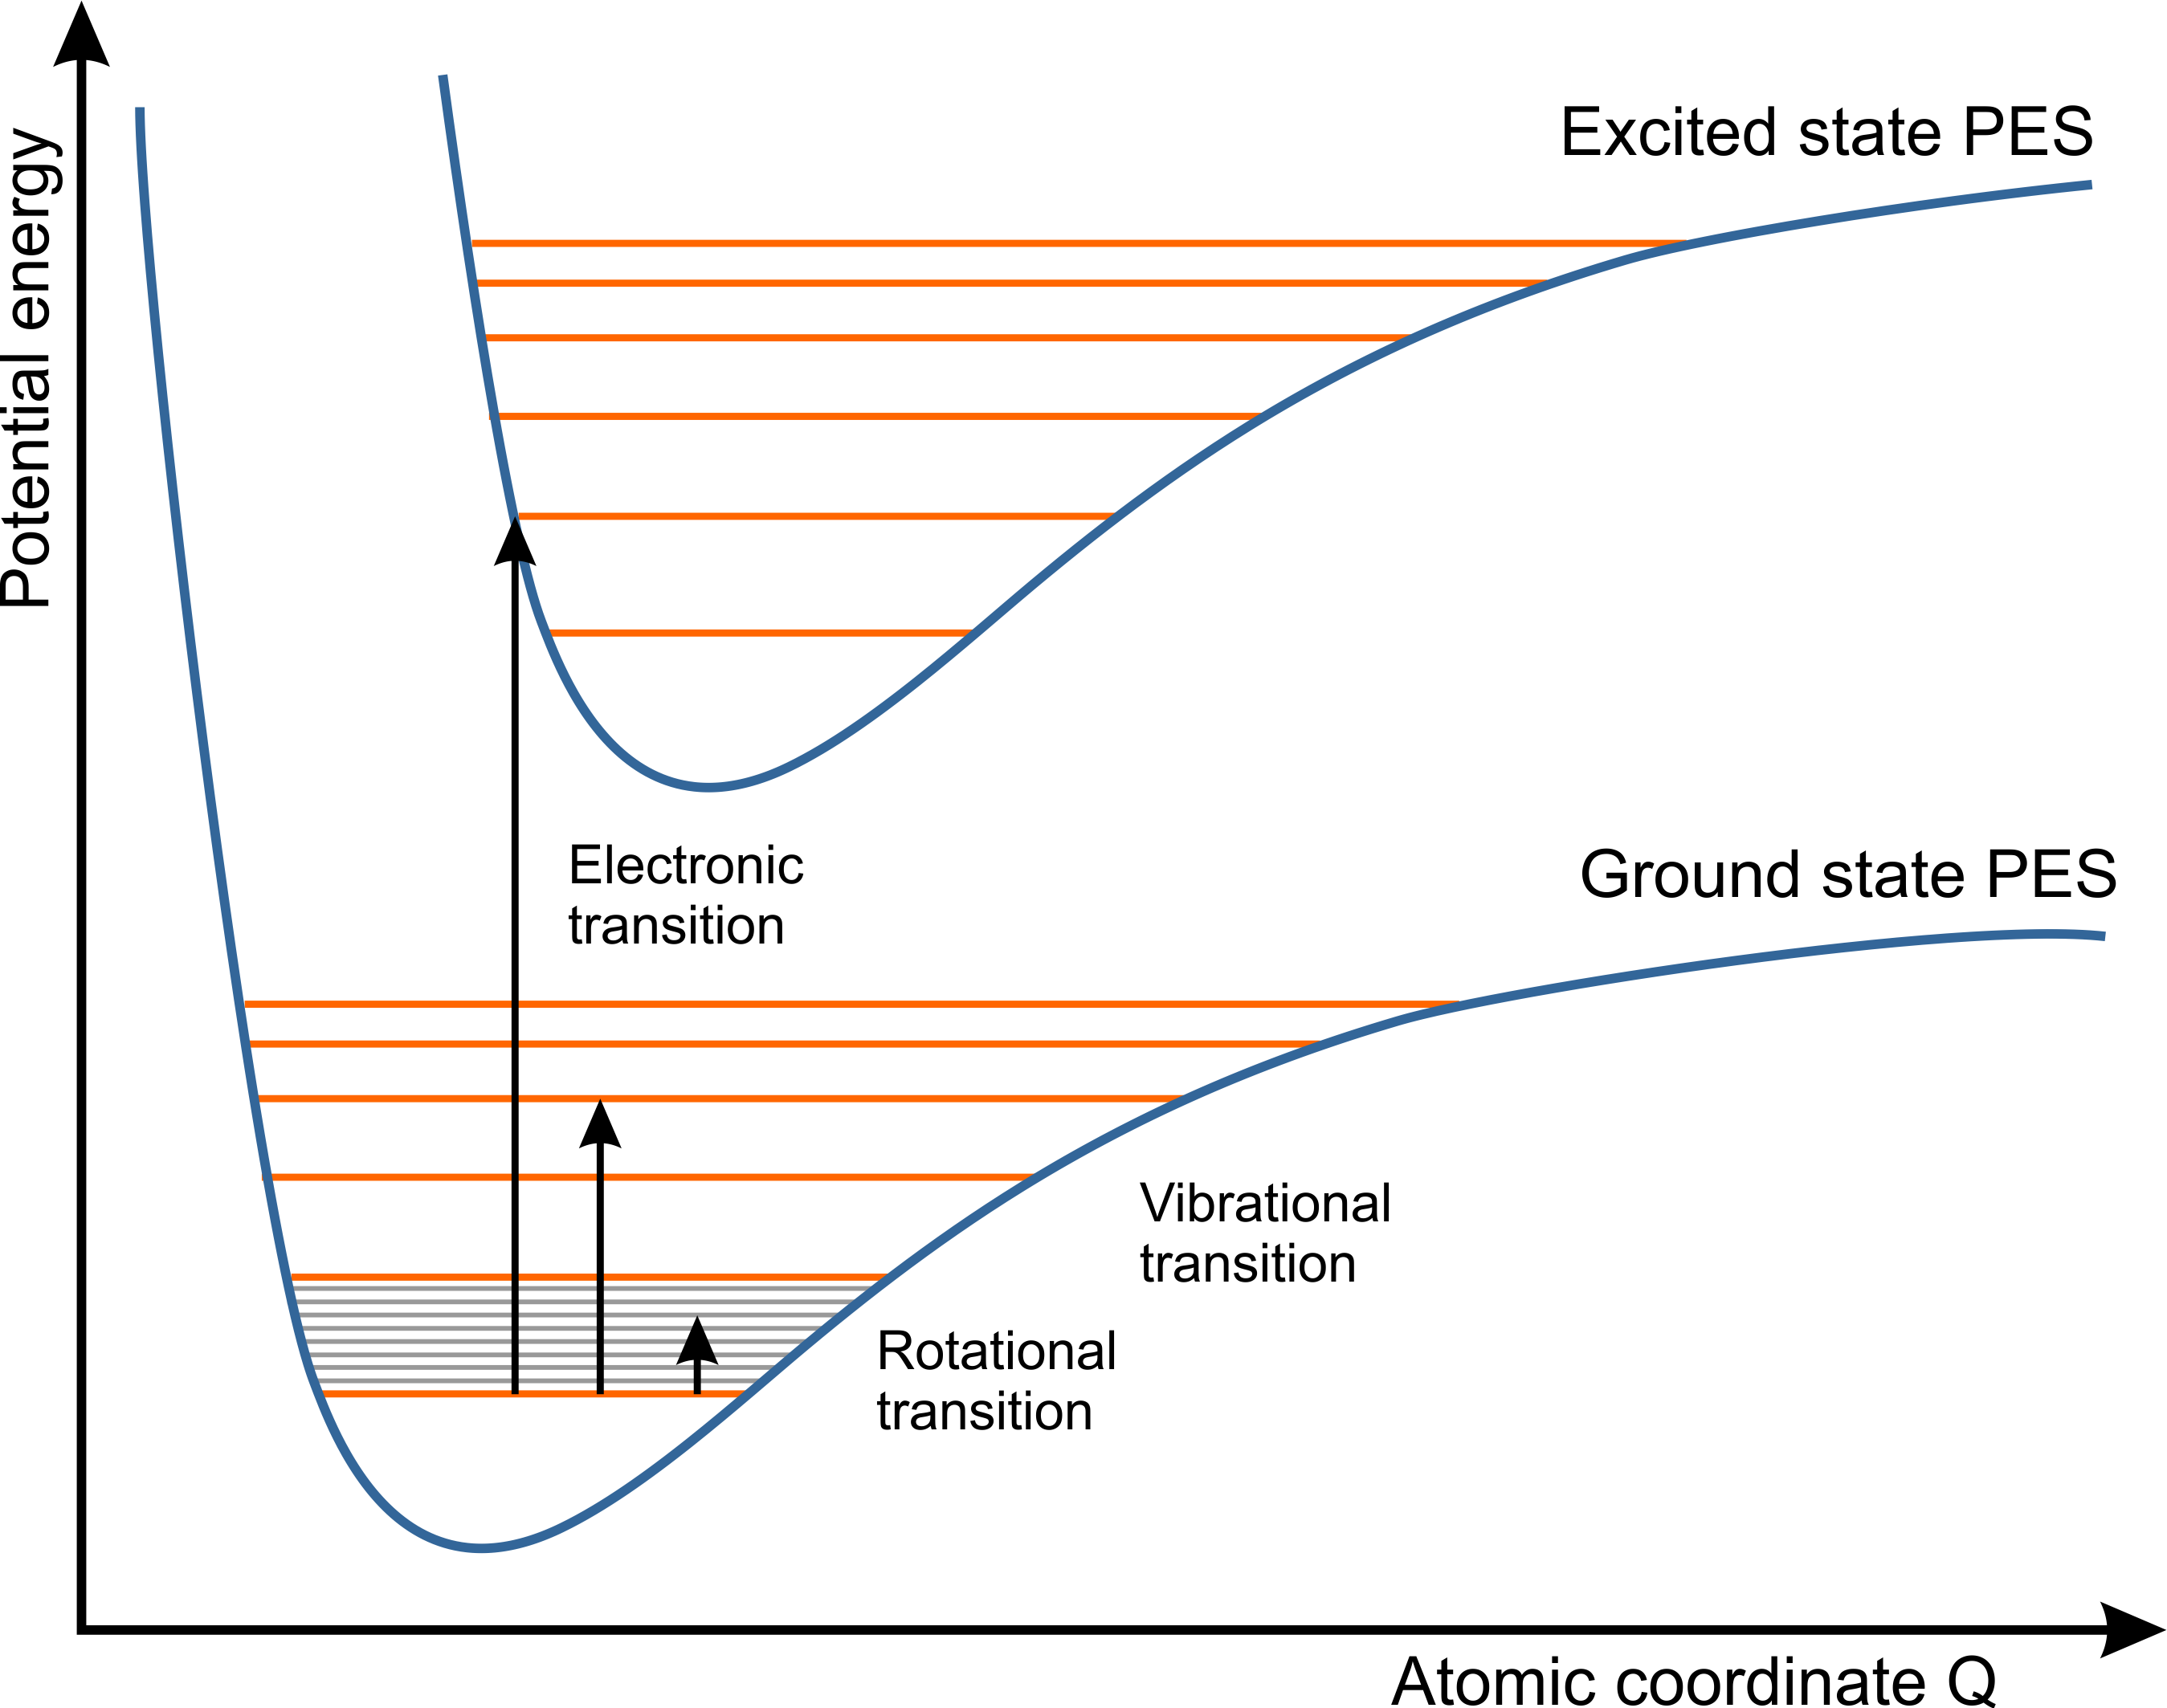
\includegraphics[width=1.0\textwidth]{BO-approx}
	\caption{The two lowest PES in the BO approximation for a diatomic molecule. In blue, the electronic PES for the ground state and first electronic excited state (UV--Vis transition). In orange, the vibrational energy levels (IR transitions), in grey the rotational levels (microwave transitions.}
	\label{fig:BO-approx}
\end{figure}

For all calculations performed in this work, we rely on the so--called Born--Oppenheimer (BO) approximation \cite{Born1927}. In this treatment, nuclei are considered as classical points which move in the potential energy surface generated by the electrons (Figure \ref{fig:BO-approx}). This way, to each nuclear configuration a corresponding electronic energy can be assigned, and nuclear coordinates enter in the Schr\''{o}dinger equation only as parameters, allowing to construct a BO surface, or PES. This approximation holds since nuclei are much slower than electrons, therefore the motion of electrons is instantaneous from the nuclei point of view. 
This approximation does not always hold, especially when dealing with light nuclei such as hydrogen. In these cases, nuclear quantum effects can have an impact on the measured properties \cite{Ceriotti2016}. In most cases, the electronic ground state is also not interacting with the higher electronic states because of the high energy difference. In the BO approximation, the electronic energy levels are also considered fully separated and do not interact with each other. For this reason, the approximation is also called adiabatic approximation. Additional interactions have to be considered when two surfaces lie close to each other, for instance in the neighborhood of conical intersections. 

\subsection{Force Fields}

\begin{figure}[!htbp]
	\centering
 	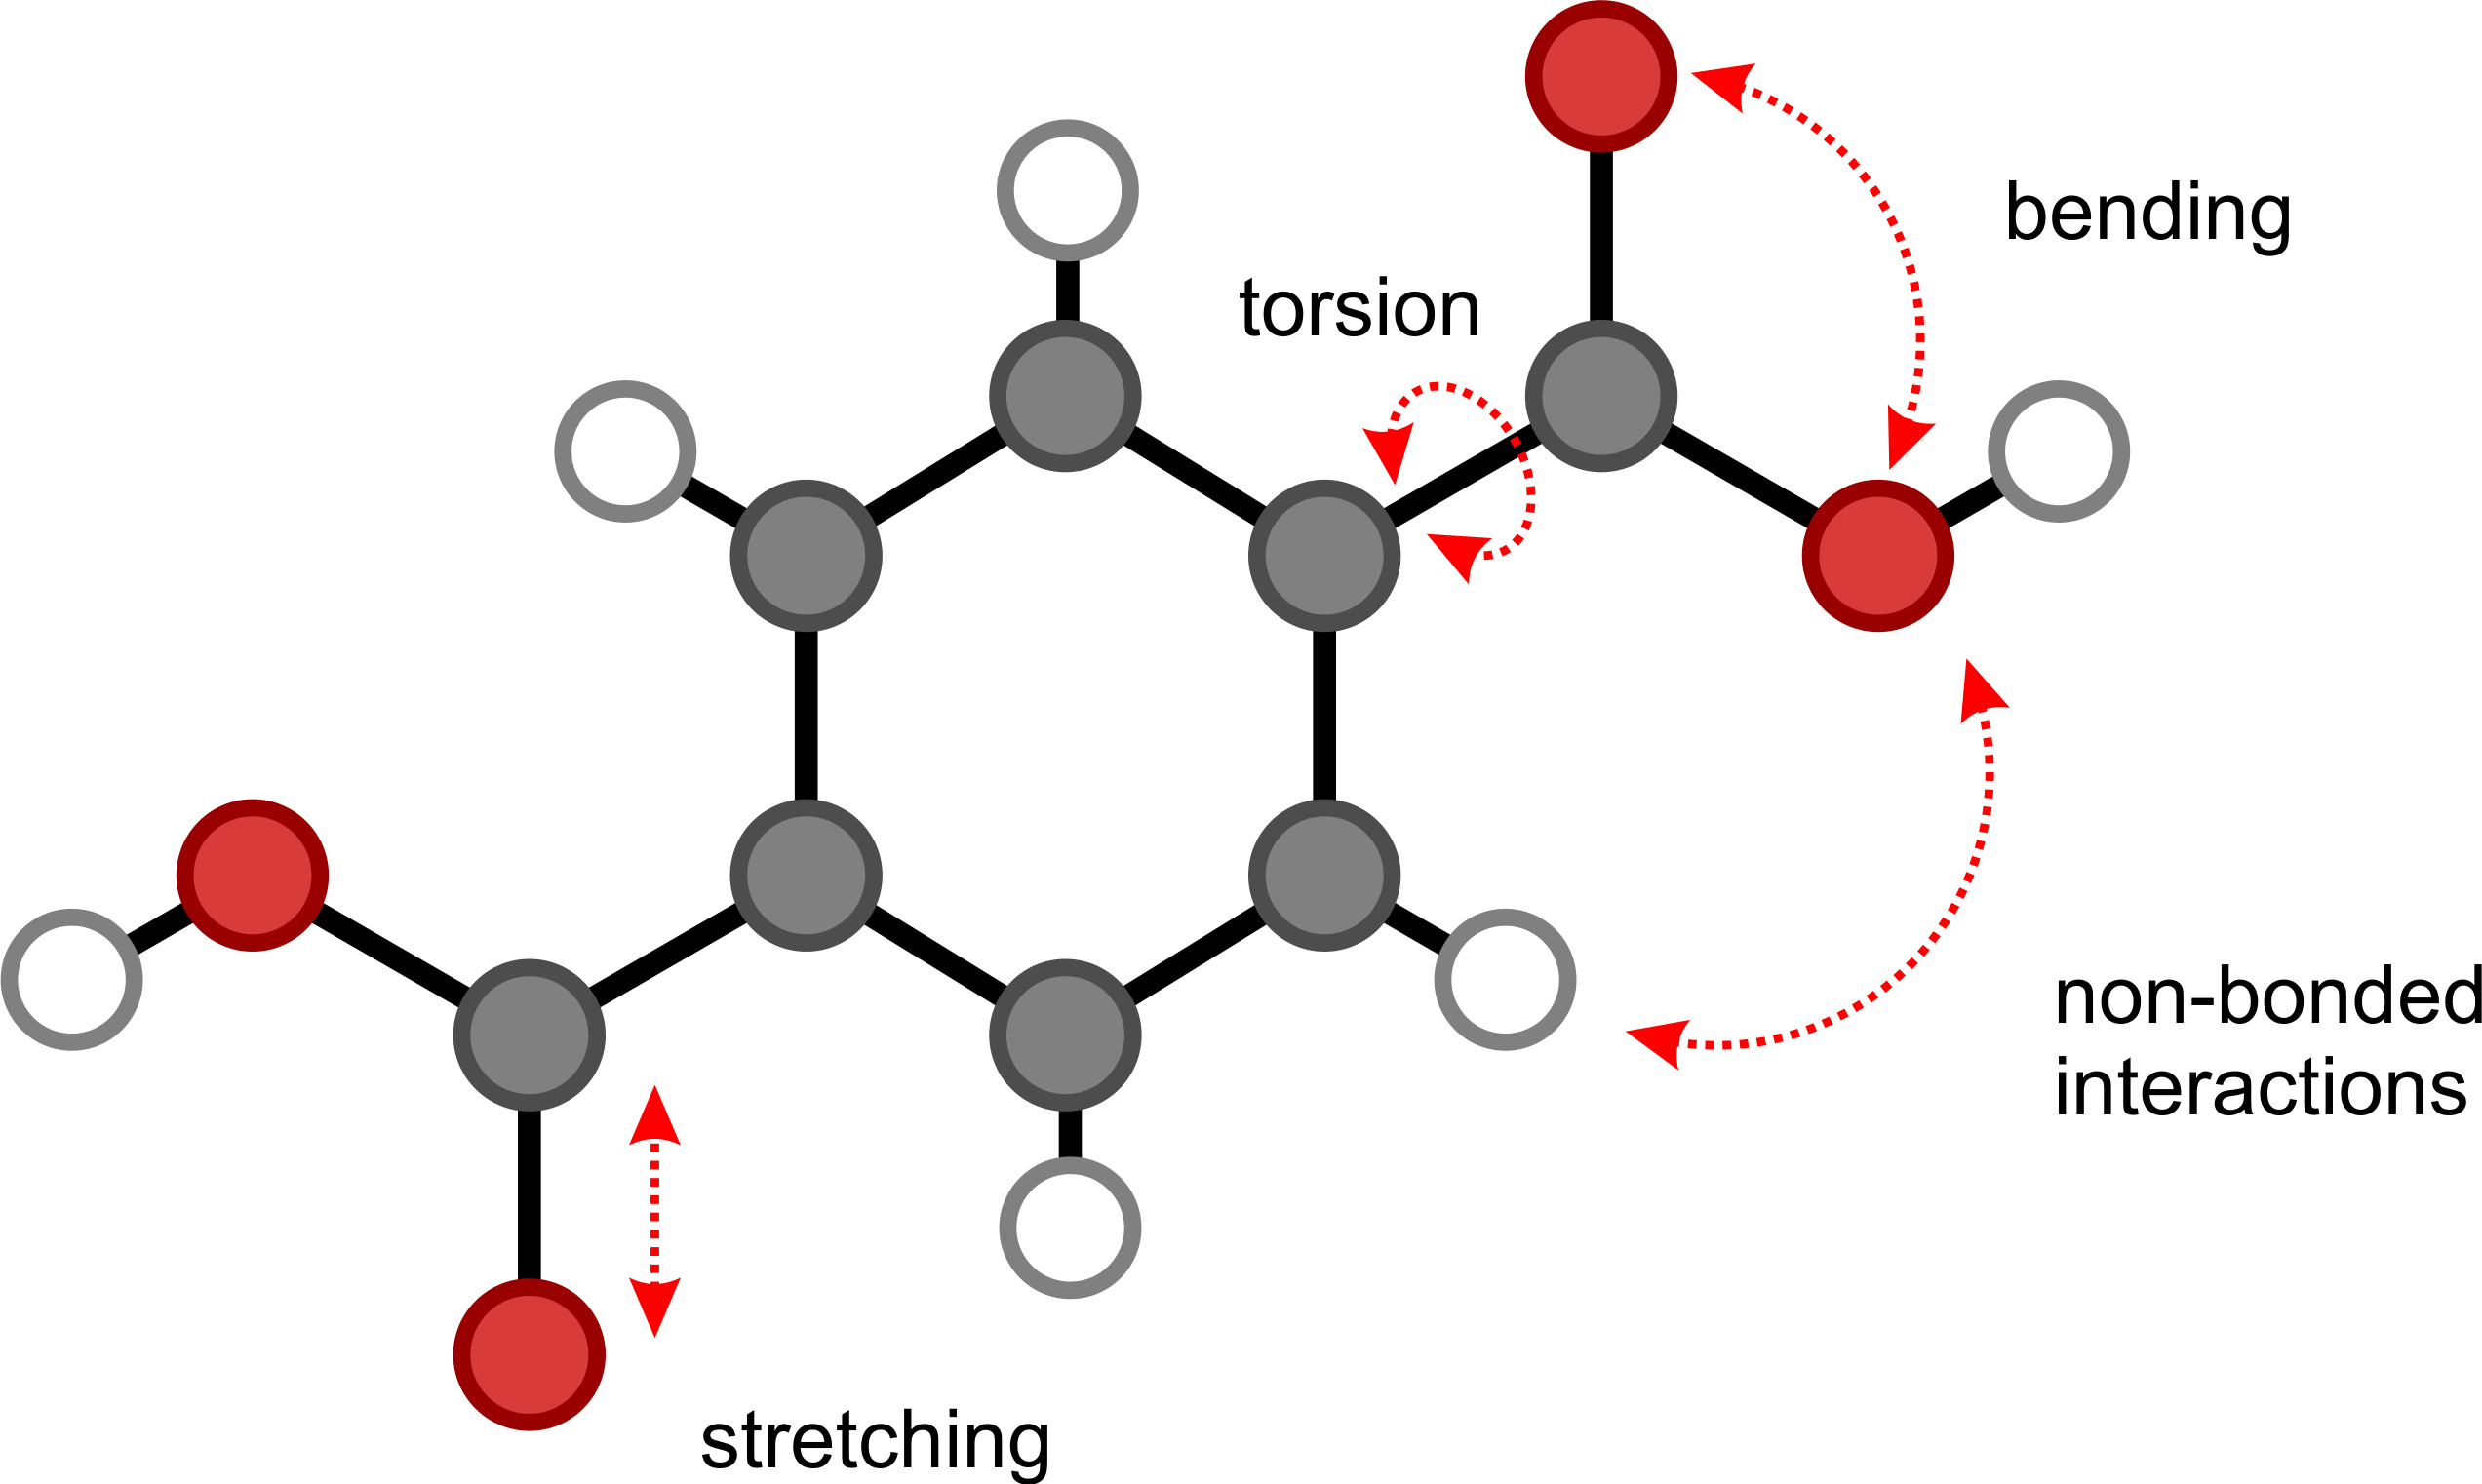
\includegraphics[width=0.5\textwidth]{forcefield}
	\caption{Representation of some of the molecular modes taken into account in a generic force field model.}
	\label{fig:forcefield}
\end{figure}

The simplest way to describe interactions between atoms which determine the PES is the so--called ``balls and springs'' model. In this treatment, all interactions are represented by interatomic classical potentials which are parametrized to reproduce the results of more accurate quantum mechanical calculations. In this work, generic force field calculations have been used in some cases to give preliminary input structures for more costly \textit{ab initio} calculations, through which the description of chemical transformations is possible. 
Force fields are often constituted by harmonic potentials which do not allow bonds being broken and formed (Figure \ref{fig:forcefield}). Reactive force fields, such as ReaxFF \cite{VanDuin2001} are currently being developed, but their application in complex heterogeneous reactions is still an ongoing chemical challenge and is out of the scope of this work. For this reason, the description of reactive processes needs a more advanced treatment, where electronic distributions are explicitly taken into account.

\subsection{Density Functional Theory}
Density functional theory (DFT) has become the method of choice for the study of chemical systems, due to its good trade--off between computational cost and accuracy of the obtained results. DFT began in the 1920’s with the work of Thomas and Fermi \cite{Thomas1927, Fermi1928}, but it was only in the ’60s that it became a complete and accurate theory, shown in the work of Kohn, Hohenberg and Sham\cite{Hohenberg1964}. The fundamental property that DFT describes is electron density as opposed to many body electron wavefunctions, which allows to reduce enormously the number of variables in the case of complex systems. Two fundamental theorems by Hohenberg and Kohn state that there is a unique relation between electronic density and total wavefunction, therefore the ground state density allows us to determine all properties of the system. Moreover, the ground state density can be obtained from a minimization of the total energy functional with a variational method by solving the so--called Kohn--Sham equations. The global minimum value of the functional determines the exact ground state of the system. This way it is possible to obtain the total energy of the system and the forces which act on the atoms, two quantities which are needed in all the simulations performed in this work. 
\npar
In principle, DFT is an exact method, but the minimization of energy is far from trivial. Kohn and Sham \cite{Kohn1965} introduced a method which replaces the many--body problem with an auxiliary system of non--interacting particles, allowing a fast solution of the eigenvalue problem. What needs to be added in this treatment is an additional functional which describes exchange and correlation. Nowadays one of the greatest challenges in DFT consists in the search for an accurate expression for the exchange--correlation functional.
The simplest method is known as Local Density Approximation (LDA) initially proposed by Kohn and Sham \cite{Kohn1965} and can also be adapted to include spin in the Local Spin Density Approximation (LSDA) \cite{Vosko1980}. A more refined method is the Generalized Gradient Approximation (GGA) which involves the calculation of the gradient of electron density and includes functionals such as B88 \cite{Becke1988}, LYP \cite{Lee1988} and PBE \cite{Perdew1996, Perdew1997}, used in this thesis. 
 More recent functionals are the so--called hybrid functionals, which include the Hartree--Fock (HF) exchange, such as B3LYP \cite{Becke1988, Becke1993, Lee1988}, which is a combination of B88, LYP and LDA with HF, and PBE0 \cite{Adamo1999}, which mixes PBE with HF. These functionals can give a more accurate electronic description of the system but are computationally very expensive. As compromise between accuracy and computational cost is a geometry optimization with PBE, and a single point calculation to refine the energies with B3LYP, as performed in \textbf{PAPER I}.

\subsubsection{Dispersion interactions}
In this thesis we often encounter noncovalent interactions which need to be treated with high accuracy, such as the adsorption of guest molecules on the zirconium Lewis acid sites or interaction between solvent molecules. One of the challenges of DFT methods is the description of long range dispersive interactions such as London forces, which are commonly referred to as van der Waals interactions. These interactions are due to many particle electron correlation effects which are present also in absence of charges and can have a significant impact on the noncovalent interaction energy. To tackle this problem, various dispersion schemes have been proposed. One of the most used is currently the Grimme--D3 method \cite{Grimme2010}, where a damped $-C_{6}R^{-6}$ function is added to the DFT functional. Recently, more advanced dispersion schemes have been developed, such as the many body dispersion scheme \cite{Buko2016}, or the one of Tkatchenko and collaborators \cite{Ambrosetti2014}, although for the systems we are studying not many benchmarks of these new methods have been performed so far \cite{Wieme2018}.

\subsection{Geometry optimization}
In order to obtain molecular structures that have physical significance and their relative energies, the arrangement of the atoms needs to be optimized. There are generally two types of molecular structures that we need to find in our simulations, the equilibrium geometries, which correspond to \textit{minima} of the PES, and the transition state geometries, which correspond to first order saddle points, as displayed in Figure \ref{fig:PES}. These points are characterized by null first derivatives of the energy (the total forces acting on each atom are sufficiently close to zero), all positive second derivatives for local \textit{minima} and one negative second derivative for first order saddle points, which correspond to transition states. 

\begin{figure}[!htbp]
	\centering
 	\includegraphics[width=1.0\textwidth]{PES}
	\caption{Schematic representation of the potential energy surface and the stationary points.}
	\label{fig:PES}
\end{figure}

The geometrical optimization of reactants and products consists in a minimization of the energy along the nuclear coordinates. Often the starting point is the experimental structure which can be obtained from diffraction data. In the most used codes several minimization methods are implemented, each characterized by a different computational cost and robustness, such as steepest descent, conjugated gradient or simulated annealing. The algorithms will find local \textit{minima}, and do not guarantee that the system will be in a global \textit{minimum}, therefore the minimizations must start from a sufficiently good guess. 
\npar
The search for transition states is far from trivial and often requires an iterative procedure involving different methods and requiring a good knowledge about the system and chemical process under study. In the calculations performed in this thesis, we often start from an equilibrium structure and as a first guess, we adapt the bond lengths and angles to be close to the transition state with a molecular editor such as Zeobuilder \cite{Verstraelen2008}. These bond lengths are then fixed, and the rest of the structure is reoptimized. The Hessian of this partly optimized structure needs to be then computed, and the vibrational modes analyzed, to check which (if any) negative frequency corresponds to the transition state. The system can be optimized again without the constraint using an improved dimer method along a selected eigenvector \cite{Heyden2005} which is followed by the optimization with a \textit{quasi}--Newton method \cite{Press1989}. In some difficult cases, the TS search can be initiated on simpler cluster models and optimized in a code in which methods are usually implemented to directly find the TS structure. This way, a first guess of the TS geometry might be obtained and further transferred to the periodic model. In both transition states and \textit{minima}, if there are superfluous negative frequencies, these need to be removed. Often, it is sufficient to minimize the energy along that vibrational mode. Single point energy calculations can be performed for different values of the displacement along that mode, and the lowest point in energy can be used as starting point for a subsequent minimization of all the coordinates.

\subsubsection{Cell optimization}
In the case of periodic systems, not only the structure, but also the unit cell needs to be optimized. This is not trivial, as when using a finite plane wave basis set the number of plane waves depends on the volume of the unit cell. If the volume changes during the optimization, artificial forces which go under the name of Pulay stress can arise. This would require many iterations to optimize the volume. In this thesis, another approach was used \cite{Vanpoucke2015} which relies on an equation of state fit. For a given volume, for instance taken from experimental data, the unit cell is optimized. Then a set of equally spaced different volumes is defined and for each of these points the geometry and unit cell parameters are optimized. This way it is possible to construct an energy--volume curve, which for a rigid system can be fitted with a Birch--Murnaghan equation of state \cite{birch1947finite,murnaghan1944compressibility}, allowing to extract the volume $V_0$ which corresponds to the \textit{minimum} electronic energy $E_{0}$. 
\[
E(V) = E_{0} + 
\dfrac{9V_{0}B_{0}}{16}
\left\lbrace 
\left[\left(\dfrac{V_{0}}{V}\right)^{\frac{2}{3}} - 1\right]^{3} B'_{0} +
\left[\left(\dfrac{V_{0}}{V}\right)^{\frac{2}{3}} - 1\right]^{2}
\left[6 - 4\left(\dfrac{V_{0}}{V}\right)^{\frac{2}{3}}\right]
\right\rbrace
\]
Where $B_0$ and $B'_{0}$ are the bulk modulus and its derivative. A new structure is then generated at this given volume and coordinates and unit cell parameters are optimized again.

\subsection{Molecular vibrations}
As seen in the previous paragraph, for many purposes in this thesis we need to calculate the second order derivatives (Hessian matrix) of the PES, which are associated to molecular vibrations. First of all, the Hessian gives us information about the curvature of the surface and the nature of the stationary points encountered during the minimization. The second order derivatives are obtained by displacing the atoms in the three directions and calculating the energies, then the Hessian is diagonalized to determine the eigenvectors that correspond to the vibrational motions. 
From the Hessian we can calculate the vibrational frequencies, which open the door to a lot more information on the system than a single point calculation. As a matter of fact, single point calculations are performed at 0 K, but even at this temperature nuclei vibrate around their equilibrium positions, and this movements are responsible for vibrational entropy. We can approximate these motions with those of harmonic oscillators, by using the vibrational frequencies constructed from the Hessian. 
\npar
These frequencies can then be used to estimate the value of the vibrational entropy at finite temperatures, as will be explained later. In the calculations performed in this thesis, due to computational limits, a partial Hessian approach (PHVA) was used when dealing with reactions, as implemented in the TAMkin toolkit \cite{Ghysels2010}. The quantity that needs to be derived from these calculations is the change in free energy, which mainly depends on the parts of the system that change during the reaction, in the case of a heterogeneous catalyst the active site and the adsorbed reactants. Therefore, restricting the entropy calculations only to this part of the system is a good approximation that allows to decrease enormously the computational cost \cite{Ghysels2007}. This approach has been used in the calculation of the free energy barriers for the Fischer esterification on UiO--66 (\textbf{PAPER I}), where the atoms taken into account were the adsorbed reactants and four atoms of the active sites in their immediate proximity, as displayed in Figure \ref{fig:PHVA}.

\begin{figure}[!htbp]
	\centering
 	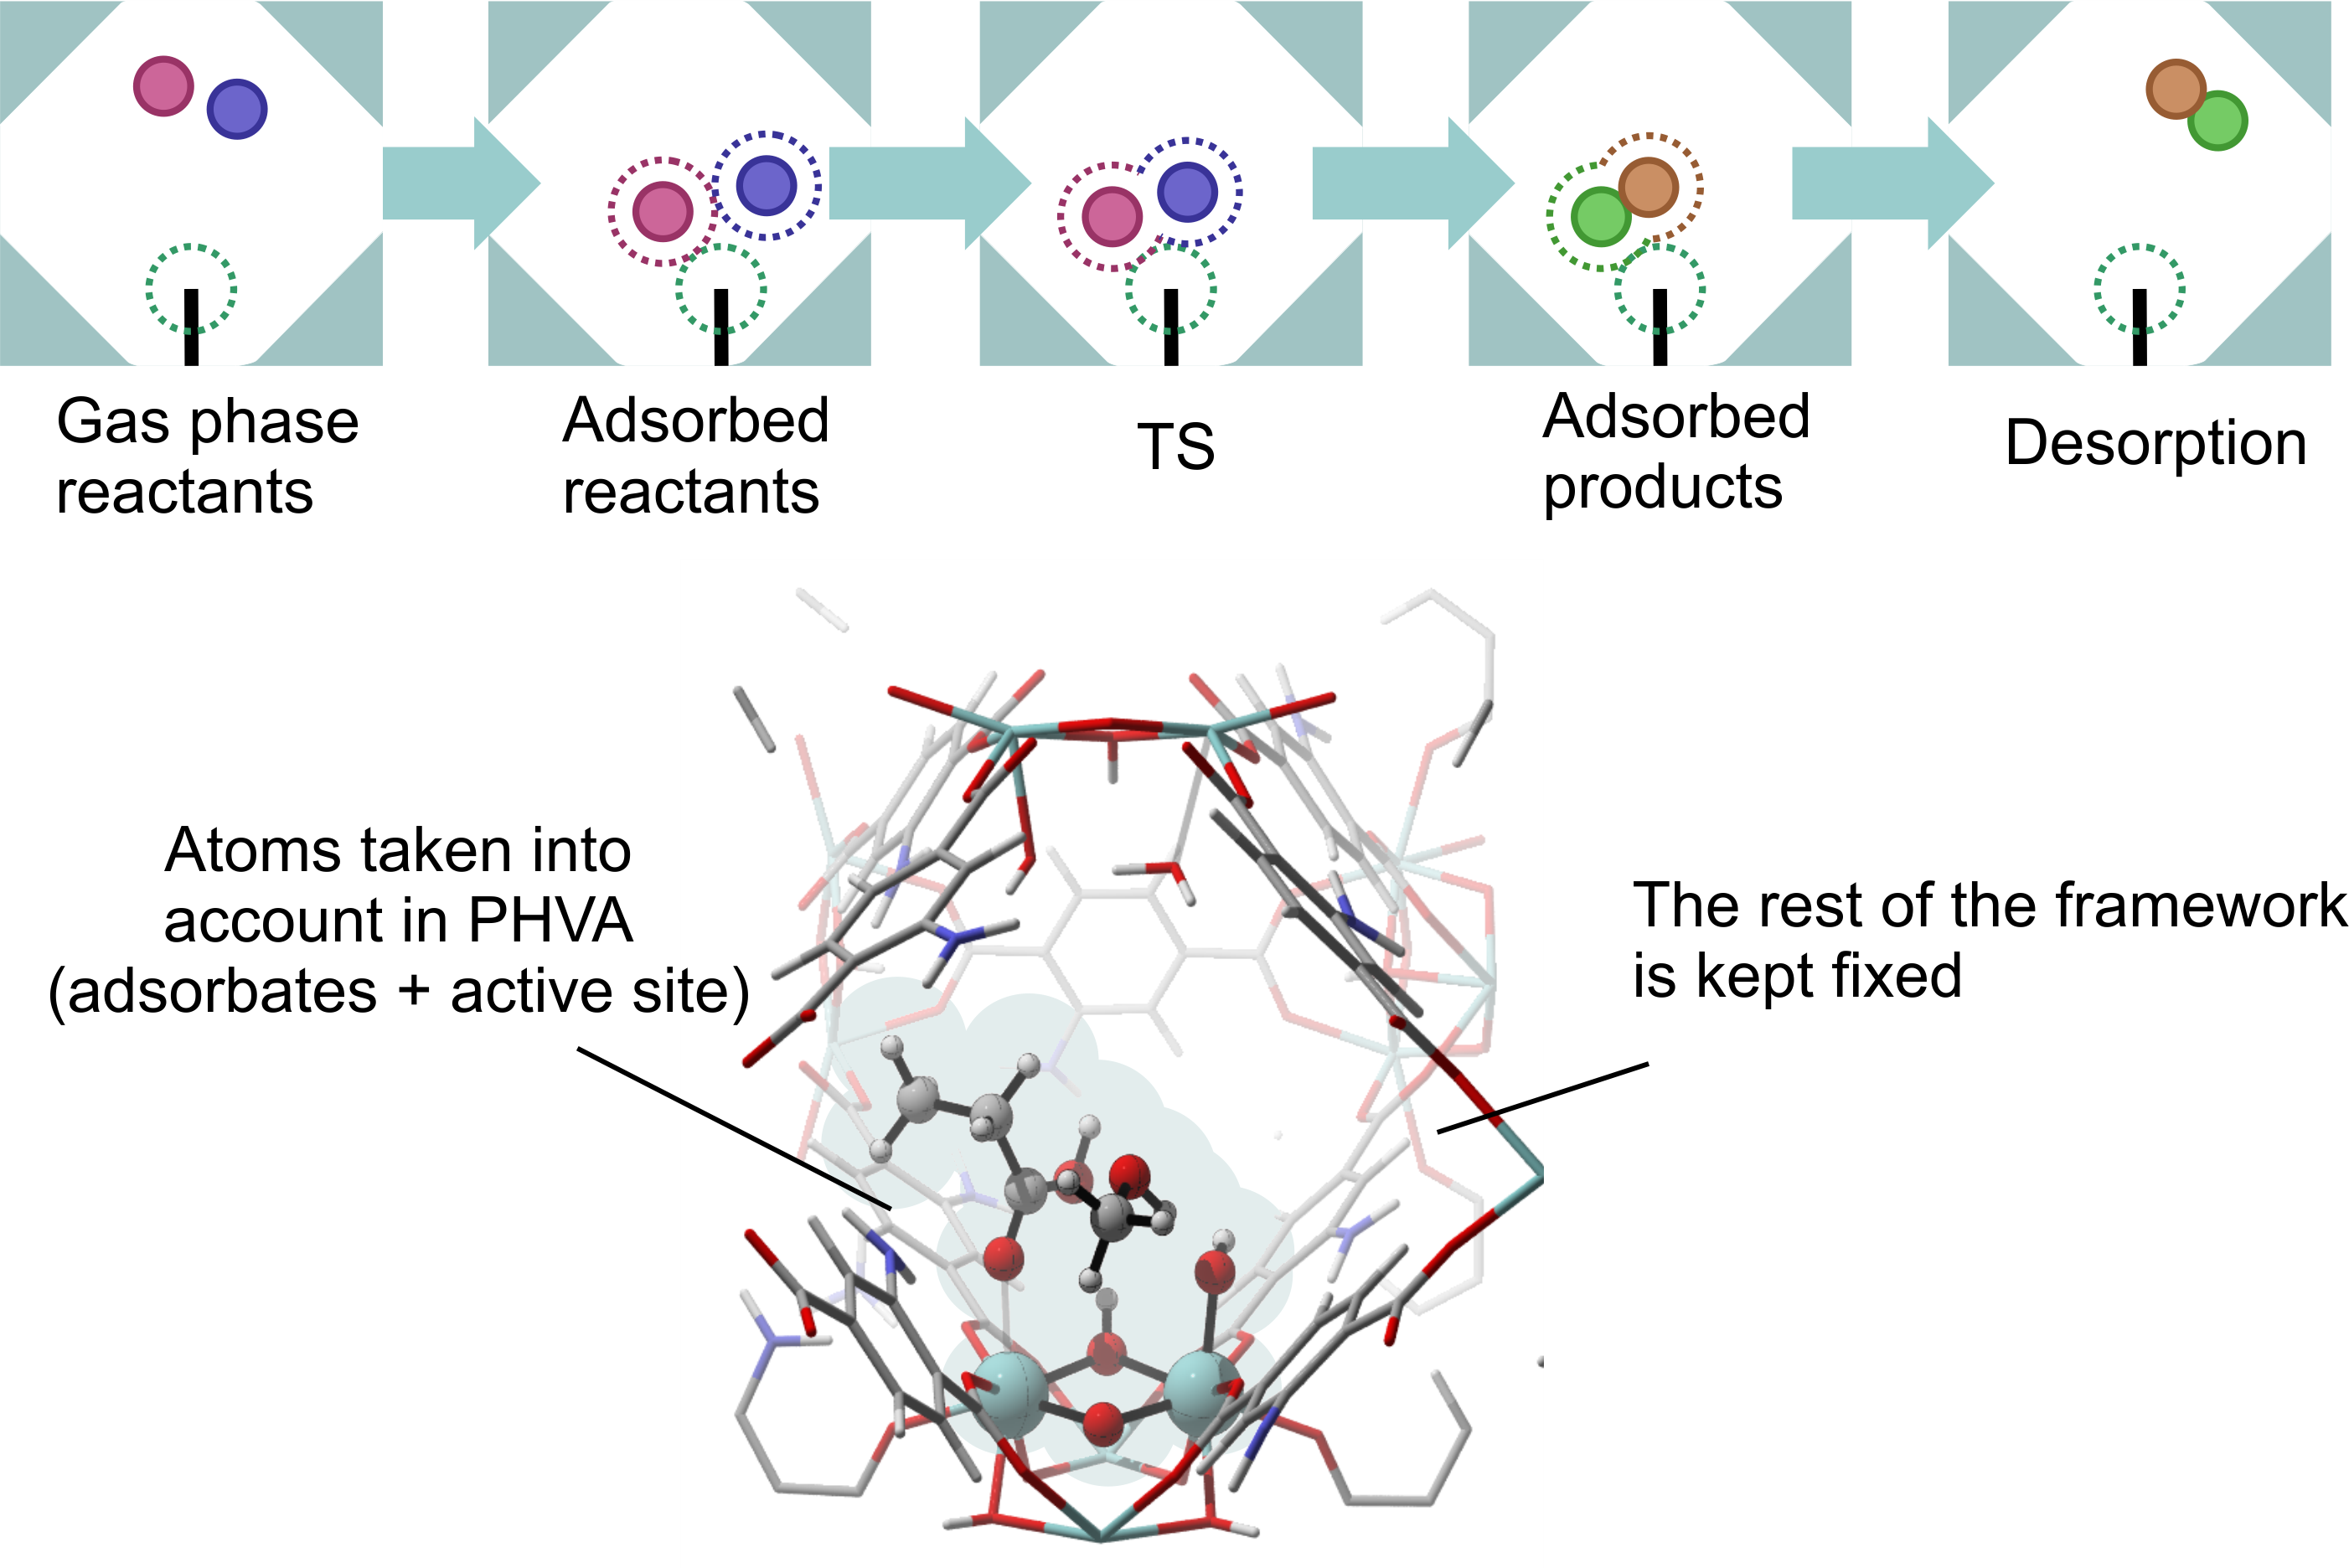
\includegraphics[width=1.0\textwidth]{PHVA}
	\caption{representation of the atoms taken into account in the PHVA approach. Top: a schematic representation of a reactive process in nanoporous material, bottom: a snapshot from the static calculations where the atoms of the active site and the adsorbates are highlighted}
 \label{fig:PHVA}
\end{figure}

\section{Free energy}
The central thermodynamic quantity that determines the outcome of a reaction is the free energy change associated to the process. In general, a chemical system will undergo changes in a direction that minimizes its free energy, until an equilibrium is reached. Knowing the difference in free energy between reactants and products allows us to know the equilibrium constant for a given reaction. The Gibbs Free energy can be decomposed in an enthalpic and an entropic contribution, that can be evaluated from the simulations knowing the molecular partition functions. Initially, the total internal energy $U$ has to be obtained from the electronic energy $\varepsilon_0$, the zero--point vibrational energy $E_{ZPE}$ and the molecular partition function $Q$ at constant number of particles $n$ and volume $V$:
\[
U = U_{0} + R T^{2}\left(\frac{\partial \ln Q}{\partial T}\right)_{n,V}
\]
\[ U_{0} = \varepsilon_{0} + E_{ZPE} \]
Where $R$ is the gas constant, equal to the product $N_{A}\cdot k_{B}$ between Avogadro's number and Boltzmann constant. The molecular partition function $Q$ can be split in its translational, rotational, and vibrational components:
\[
Q = Q_{trans}Q_{rot, ext}Q_{vib}
\]
The enthalpy $H$ corresponds to the total energy plus the work associated to the change in volume.
\[
H = U + p_{0}V
\] 
%H = U + p_{0}V = U + R T
The entropy $S$ can be directly obtained from the partition function:
\[
S = R \ln Q + RT \left(\frac{\partial \ln Q}{\partial
T}\right)_{n,V}
\]
Finally, the Gibbs free energy $G$ will be:
\[
G = H - TS = U_{0} + p_{0}V - RT\ln Q
\]
Where in the case of non--interacting particles $p_{0}V = RT$ following the ideal gas law. We can therefore define a free energy surface (FES) that is function of coordinates of the system, and can be derived from the PES.

\subsection{Equilibrium}
As explained above, there is a tight connection between free energy and equilibrium concentrations in chemical reactions. As an example, an equilibrium which is of utmost importance in chemistry is the acidic dissociation of species in aqueous solution:
\[
\ce{HA + H2O <=> A- + H3O+}
\]
The acidic dissociation constant ($K_a$) is an important equilibrium constant in chemistry and is equal to the ratio between the concentration of products and reactants when the reaction reaches the equilibrium. It is often reported with its negative decimal logarithm as $pK_a$.
\[
K_a=\dfrac{\ce{[A- ][H+ ]}}{\ce{[HA]}} 
\]
The equilibrium constant is equal to the Gibbs free energy change from reactants to products.
\[
\Delta G = RT \ln K_a
\]
\[
pK_a = \dfrac{\ln 10}{RT} \Delta G
\]
Therefore, knowing the Gibbs free energy difference between reactants and products, we can have important information about the equilibrium composition of a chemical system. However, kinetic factors can sometimes play a major role, and equilibrium cannot always be easily reached.

\subsection{Transition state theory}
A chemical reaction is a process that through rearrangement of the atoms transforms one stable state into another. Every elementary reaction can be represented as a minimum energy path connecting two \textit{minima} along the FES. Furthermore, along this reaction path the existence of a saddle can be postulated, which is the highest point in energy that needs to be crossed to go to the product state. 
The saddle point is typically called transition state or activated complex and it is the basis for the transition state theory (TST) developed by Eyring in the 1930’s, one of the most successful chemical theories which allows to explain reaction rates of elementary chemical reactions. The assumption of the theory is that there is a \textit{quasi}--equilibrium between reactants and activated complex, and the rate constant can be obtained by the size of the energy barrier and by the frequency at which the system can cross the barrier. This is possible because the barrier acts as a bottleneck in the reaction, its crossing is a rare event and all the kinetics depends only on it. For a unimolecular reaction, the rate constant can be derived from the partition functions of reactant, TS and their energy difference:
\[
k(T) = \dfrac{{k_B T}}{h}
\dfrac{{q_{TS,\ddagger}}}{{q_R}} e^{- \frac{\Delta E^{\ddagger}}{k_B T}}
\]
Where $k_B$ is the Boltzmann constant, $h$ is the Planck constant, $q_R$ and $q_{TS,\ddagger}$ are the molecular partition functions of reactants and activated complex for all coordinates except the reaction coordinate, evaluated from the zero--point vibrational level. 
\[
q_{vib,i} = \prod_{i=1}^{N_{dof}} \dfrac{1}{1 - e^{- \frac{h \nu_{i}}{k_B T}}}
\]
Where $N_{dof}$ is the number of vibrational degrees of freedom of the system. The energy difference $\Delta E^{\ddagger}$ includes electronic energy and zero--point vibrational energy difference at 0 K:
\[
\Delta E^{\ddagger} = E_{0}^{TS} - E_{0}^{R} + \Delta E_{0,vib}
\]
\[
\Delta E_{0,vib} = \sum_{i=0}^{N_{dof}-1} \frac{h \nu_{i}^{TS,\ddagger}}{2}
- \sum_{i=0}^{N_{dof}} \frac{h \nu_{i}^{R}}{2}
\]
This theory has some limitations, and may fail in the case of labile intermediates, when nuclei deviate from a classical behavior, or at high temperatures. For a given reaction, in fact, there will be many paths characterized by different barriers, and at low temperature only the lowest one will be likely to be crossed. When the kinetic energy is high enough, many other paths will be activated. The transition state will occupy a larger region of the PES, and it will not be possible to derive entropy from the vibrational partition functions.
\begin{figure}[!htbp]
	\centering
 	\includegraphics[width=1.0\textwidth]{static-scheme}
	\caption{Static reaction profile for a reactive process with and without catalys }
	\label{fig:static-scheme}
\end{figure}

\section{Exploring the free energy surface}
Static calculations, where molecular vibrations are approximated using harmonic oscillators, can fail to give an accurate representation of the entropy when there is a high configurational freedom. When the FES is flat with respect to $k_B T$, the system at equilibrium can evolve in a larger region of the PES and move along more than one \textit{minimum}. In this case, vibrational frequencies are anharmonic and it is not possible to represent the system by approximating around one single \textit{minimum}. Therefore, static calculations are not always sufficient in describing the system at operating conditions. In this view, molecular dynamics (MD) techniques, which follow the time evolution of the system, can resolve this shortcoming.

\subsection{Ab initio Molecular Dynamics}
From MD simulations, thermodynamic properties such as free energy can be obtained taking into account a whole region of the PES instead of a single point. This is based on the ergodic theorem, that in one of its formulations states that the time average of equilibrium properties is equal to the ensemble average, in the limit of a sufficient long simulation. 
\npar
MD simulations are based on solving Newton’s equations of motion:
\[
M_i \ddot{\mathbf{R}}_i = \mathbf{F}_i = - \nabla_i V
\]
where $M_i$ and $\mathbf{R}_i$ are the mass of a given nucleus and its coordinates, $\mathbf{F}_i$ the forces that act on it, which correspond to the gradient $\nabla_i V$ of the PES. There are many ways to calculate these quantities and to integrate the equations of motion, and at present time, chemists and physicists can choose between a plethora of MD techniques which span a whole range of complexity, accuracy and computational cost. 
In the calculations performed in this thesis, potential energy and forces on the PES are calculated from first principles by means of DFT to account for the full dynamic behavior of the material by ab initio molecular dynamics (AIMD). The calculation of electronic properties which define the PES is decoupled from the propagation of nuclear motions, in a method called Born--Oppenheimer Molecular Dynamics (BOMD). Other famous AIMD methods, which differ by how the calculations of electronic potential and the equation of motion are combined, are the Car--Parrinello MD (CPMD)\cite{Car1985}, where a fictitious electronic kinetic energy is added to the lagrangian, or the Ehrenfest MD, based on the namesake theorem \cite{Ehrenfest1927, Marx2009}. 
\npar
The first MD calculations were performed in the microcanonical (NVE) ensemble, where total energy, number of particles and volume are fixed. However, in experiments it is often the temperature that is fixed, not the energy. In general, the choice of the ensemble depends on the thermodynamic quantities that need to be determined. Nowadays there are many thermodynamic ensembles in which the simulation can be performed. The most convenient for a comparison with experiments are the canonical (NVT), with fixed number of molecules, volume and temperature, or the isothermal--isobaric (NpT), with fixed number of molecules and temperature, but where the volume can fluctuate. In order to have a fixed average temperature, some control of the kinetic energy of the atoms is needed. Various thermostats, which differ in terms of speed and robustness, are implemented in every MD code. In this thesis, Nose’--Hoover thermostat was used, where the system is connected to a heat bath. The pressure is also controlled in simulations by means of a barostat. The most commonly used is the one developed by Martyna, Tobias, and Klein (MTK)\cite{Martyna1994}.

\subsubsection{Radial distribution functions}
From MD trajectories, different macroscopic properties can be derived. An important structural property is the radial distribution function (RDF) or pair correlation function $g(r)$, that describes the probability density between specific atoms as a function of the distance, normalized with respect to a probability distribution of a homogeneous gas with the same density. The RDF can be calculated from the following expression:
\[
g_{ij}(r) = \dfrac{dn_{ij}(r)}{4\pi r^2 dr \rho_i}
\]
where $dn_{ij}/dr$ represent the number of atoms of type $j$ within a certain distance of the atoms of type $i$, and $\rho_i = V / N_i $ represent the density of the homogeneous distribution. The integral of the RDF can also give valuable insight into the number of atom pairs at a given distance, such as what is the average coordination of a certain chemical species.

\subsubsection{Vibrational density of states}
Information on the time evolution of certain quantities in the system can be obtained by calculating time autocorrelation functions. The correlation of a certain variable with itself is equal to:
\[
\left\langle X(0):X(t)\right\rangle = \lim_{N \to \infty} \dfrac{1}{T}\int_{0}^{T}X(t)X(t+\tau)d\tau
\]
Autocorrelation functions offer a measure of the response of the system to a given stimulus, which is function of the density of states. The response of a system to a perturbation is equal to the power spectrum of the autocorrelation function of the fluctuations of the involved observable\cite{kubo1957statistical}. For instance, by calculating the power spectrum of the atomic velocities autocorrelation function, we can obtain the vibrational density of states, as done in \textbf{PAPER IV}. These spectra contain all the dynamic and anharmonic information that is neglected in the static frequency calculations.

\subsubsection{Towards modeling at operating conditions}
With the growth in computational time, the new challenge is constituted by modeling the system at operating conditions. Many chemical reactions, especially when performed at mild conditions, involve the presence of a solvent. In order to move closer to modeling the system at operating conditions, the solvent in the pores can also be taken into account. This adds a lot of degrees of freedom to the system, and for this reason often an implicit description of the solvent is done, such as in the Periodic Continuum Model (PCM)\cite{cances1997new}. In the case of the work in this thesis, however, it is necessary to fully model the solvent molecules, as they are actively involved in proton transfers. To do so, the number of solvent molecules that can fit in the unit cell needs to be estimated. Monte Carlo method (MC) is an alternative approach to MD to explore the PES for complex systems. It was initially developed for the calculation of multidimensional integrals and is nowadays largely used in chemistry, especially when dealing with adsorption. In the framework of this thesis, it has been applied in the Grand Canonical ensemble ($\mu VT$, fixed chemical potential, volume and temperature) to determine the number of solvent molecules that could fill the pores of the material at standard conditions.

\subsection{Enhanced sampling MD methods}
MD simulations can offer valuable insights into the behavior of a chemical system at equilibrium conditions. From these simulations, many properties can be extracted, such as equilibrium geometries, vibrational spectra, diffusion coefficients, structural parameters etc. Configurations associated to higher (or lower) values of potential energy will be sampled for shorter (or longer) times, and in principle, if a certain process is sufficiently sampled, based on the ergodic theorem we can know its equilibrium constant, and in turn the free energy barrier associated to it. However, chemical reactions, where bonds are broken and formed, are generally rare events that will not be sampled with a regular exploration of the PES. If the free energy barrier is high compared to $k_{B}T$, the probability that such event would spontaneously occur during the simulation time is practically none. This is especially true for complex molecular systems, in which processes occur in different time scales and that can only be simulated for a limited amount of time. For this reason, different enhanced sampling techniques have been developed to enhance the sampling of low probability regions of the free energy landscape \cite{valsson2016enhancing, laio2002escaping, sutto2012new, carter1989constrained, darve2001calculating, jarzynski1997nonequilibrium, rosso2002use, gullingsrud1999reconstructing}. Recently, enhanced sampling techniques have been successfully applied in heterogeneous catalysis to study processes at operating conditions \cite{dewispelaere2016insight, dewispelaere2015complex, vanspeybroeck2014first, cnudde2017effect, haigis2015hydrothermal, buvcko2011monomolecular, fraux2017recent}.
\npar
There are two main classes of methods that can be used to explore rare events on the free energy surface. The first class is characterized by methods that encompass all degrees of freedom and do not need any prior information on the free energy landscape between two points. Examples of these methods are Transition Path Sampling (TPS) \cite{dellago2002transition} and Replica exchange (RE) \cite{sugita1999replica}. The other class of techniques encompasses methods in which the sampling is enhanced along certain coordinates of the system, such as Umbrella Sampling (US) \cite{torrie1977nonphysical, patey1975monte} and Metadynamics (MTD) \cite{laio2002escaping}, shown in Fig. \ref{fig:dynamic-scheme}.

\begin{figure}[!htbp]
	\centering
 	\includegraphics[width=1.0\textwidth]{dynamic-scheme}
	\caption{Schematic representation of different MD techniques that can be used to explore the PES.}
	\label{fig:dynamic-scheme}
\end{figure}


\subsubsection{Choice of collective variable}
The PES is a highly dimensional surface, defined by the positions of all atoms in the system. However, often a reactive process can be described by few important coordinates called ``collective variables'' (CVs), which are projections of the high dimensional space. In fact, what can be considered a chemical configuration is an ensemble of microstates that are different in terms of absolute coordinates of each atom, but all contribute to the same macrostate. In some cases, a simple CV can represent the reaction coordinate for the process, but often the choice is not trivial \cite{rohrdanz2013discovering}. In general, choosing the right collective variable is crucial to describe the correct process. Often geometric parameters are used, such as distances, angles, dihedrals, or combinations of the latter. When studying certain processes, a switch function such as a coordination number (CN) derived from distance information is often the preferred choice. CNs represent a smart choice compared to distances, because for each pair of atoms, the coordination is zero for distances higher than a certain threshold.
\[
\mathrm{CN} =\sum_{i,j}\frac{1-(r_{ij}/r_0 )^{nn}}{1-(r_{ij}/r_0 )^{nd}}
\] 
Where CN is defined between two sets of atoms ${i}$ and ${j}$, $r_{ij}$ corresponds to the distance between atoms $i$ and $j$, and $r_0$ is a threshold distance. The exponential parameters $nn$ and $nd$ define how sharply the function behaves around the value $r_0$. In processes such as in the ones of \textbf{PAPER V}, we considered the coordination between a zirconium atom and the oxygen atoms of the solvent water. Such collective variable allows to consider the possibility that different water molecules could decoordinate and recoordinate, defining the same macrostate for a given value of the CN. We show that such processes cannot be studied by employing distances as CVs.

\subsubsection{Metadynamics}
Metadynamics (MTD) is a popular enhanced sampling method, used to overcome barriers in the free energy landscape, which was first proposed by Laio and Parrinello \cite{laio2002escaping, barducci2011metadynamics}. During MTD, a history dependent bias potential is added in the form of gaussian hills to the PES along a certain CV. This way, potential energy is added to already visited states, allowing to escape local \textit{minima} and explore different regions of the PES. When all states are sampled with equal probability, the free energy profile along the biased CV can be obtained from the added bias potential. As the bias is added, the system is able to evolve along all the other degrees of freedom. For this reason, this method can also provide insight into the mechanisms that occur during the exploration of the different regions of the CV, as has been done in \textbf{PAPER V}. 

\subsubsection{Umbrella sampling}
In the umbrella sampling method, a series of biased MD simulations are performed along the chosen CV. In each simulation, a bias potential is added to constrain the system to adopt a specific value of the CV, while it can evolve along all the other degrees of freedom. This way, the whole range of the CV can be explored. As each simulation is independent, this method is highly parallelizable. The free energy profile can then estimated by using different methods to combine the information obtained from the set of simulations, such as the weighted histogram analysis (WHAM) or the multistate Bennett acceptance ratio\cite{kumar1992weighted, torrie1977nonphysical}. Even if the CV is constrained in each simulation, this method can also offer valuable insight into the evolution of the system at different values of the CV, as has been done in \textbf{PAPER III}.
\npar
\npar
\npar
\npar
\npar
In summary, this chapter gives an overview of the many methods that have been employed to understand the properties of MOFs. Reactive processes can be studied by using a plethora of different computational techniques that differ in cost and accuracy. Cluster calculations were used for a first estimate of the energies, whereas periodic models were used for all the remaining part of this thesis. The increase in computational time allowed to include more complexity in the model, and to explicitly take into account the role of solvent and structural modifications in the material. During the time frame of this thesis, we moved from a static description of the chemical events towards modeling at operating conditions that allows to better describe and predict real processes. 
\clearpage{\pagestyle{empty}\cleardoublepage}